%% Based on a TeXnicCenter-Template by Gyorgy SZEIDL.
%%%%%%%%%%%%%%%%%%%%%%%%%%%%%%%%%%%%%%%%%%%%%%%%%%%%%%%%%%%%%

%------------------------------------------------------------
%
\documentclass{article}%
%Options -- Point size:  10pt (default), 11pt, 12pt
%        -- Paper size:  letterpaper (default), a4paper, a5paper, b5paper
%                        legalpaper, executivepaper
%        -- Orientation  (portrait is the default)
%                        landscape
%        -- Print size:  oneside (default), twoside
%        -- Quality      final(default), draft
%        -- Title page   notitlepage, titlepage(default)
%        -- Columns      onecolumn(default), twocolumn
%        -- Equation numbering (equation numbers on the right is the default)
%                        leqno
%        -- Displayed equations (centered is the default)
%                        fleqn (equations start at the same distance from the right side)
%        -- Open bibliography style (closed is the default)
%                        openbib
% For instance the command
%           \documentclass[a4paper,12pt,leqno]{article}
% ensures that the paper size is a4, the fonts are typeset at the size 12p
% and the equation numbers are on the left side
%
\usepackage{amsmath}%
\usepackage{amsfonts}%
\usepackage{amssymb}%
\usepackage{graphicx}
%-------------------------------------------
\newtheorem{theorem}{Theorem}
\newtheorem{acknowledgement}[theorem]{Acknowledgement}
\newtheorem{algorithm}[theorem]{Algorithm}
\newtheorem{axiom}[theorem]{Axiom}
\newtheorem{case}[theorem]{Case}
\newtheorem{claim}[theorem]{Claim}
\newtheorem{conclusion}[theorem]{Conclusion}
\newtheorem{condition}[theorem]{Condition}
\newtheorem{conjecture}[theorem]{Conjecture}
\newtheorem{corollary}[theorem]{Corollary}
\newtheorem{criterion}[theorem]{Criterion}
\newtheorem{definition}[theorem]{Definition}
\newtheorem{example}[theorem]{Example}
\newtheorem{exercise}[theorem]{Exercise}
\newtheorem{lemma}[theorem]{Lemma}
\newtheorem{notation}[theorem]{Notation}
\newtheorem{problem}[theorem]{Problem}
\newtheorem{proposition}[theorem]{Proposition}
\newtheorem{remark}[theorem]{Remark}
\newtheorem{solution}[theorem]{Solution}
\newtheorem{summary}[theorem]{Summary}
\newenvironment{proof}[1][Proof]{\textbf{#1.} }{\ \rule{0.5em}{0.5em}}

\begin{document}

\begin{flushleft}
\textbf{Course:} CSC 520, Introduction to Artificial Intelligence\\
\textbf{Homework 4}\\
\textbf{Student: Xusheng Xiao} \\
\textbf{Unity ID: xxiao2} \\
\textbf{Email: xxiao2@ncsu.edu}
\end{flushleft}

\noindent{\hrulefill}

\bigskip

\begin{enumerate}
  \item (20 points) Two grad students in the Knowledge Discovery Lab (KDL) prefer two different coffees (Brazilian and Indian). However, there is only one coffee machine in the lab! There are three operators: load coffee into the machine, brew the coffee, and clean the machine. Suppose the machine contains old Brazilian coffee, and a student wishes to brew a fresh pot of Indian coffee. Help the grad students with a plan!
  
The PDDL description of the actions are as follows (X is a variable; nil and waste are constants):

Action: load(X)	 \\
\hspace*{6ex} 	PRECOND: coffee(X), loaded(nil) \\
\hspace*{6ex} 	EFFECT: loaded(X), $\neg$loaded(nil)\\
Action: brew(X)	 \\
\hspace*{6ex} 	PRECOND: loaded(X), $\neg$loaded(nil), $\neg$loaded(waste)\\
\hspace*{6ex} 	EFFECT: $\neg$loaded(X), loaded(waste), pot(X)\\
Action: clean(X)	 \\
\hspace*{6ex} 	PRECOND: loaded(X), $\neg$loaded(nil)\\
\hspace*{6ex} 	EFFECT: $\neg$loaded(X), loaded(nil)\\
 	
\begin{enumerate}
  \item (5 pts.) Specify the initial state and the goal conditions, and draw the ``relaxed planning graph'' for this problem. Use $b$ and $i$ as constants to represent the coffee. (A relaxed planning graph ignores negative interactions--ie, no mutexes.)\\
  
  Init(loaded(waste) $\wedge$ coffee(b) $\wedge$ coffee(i)) \\
  
  goal(pot(i))\\
  
  Figure \ref{fig:planninggraph} shows the relaxed planning graph.
  
  %\usepackage{graphics} is needed for \includegraphics
\begin{figure}[!iht]
\begin{center}
  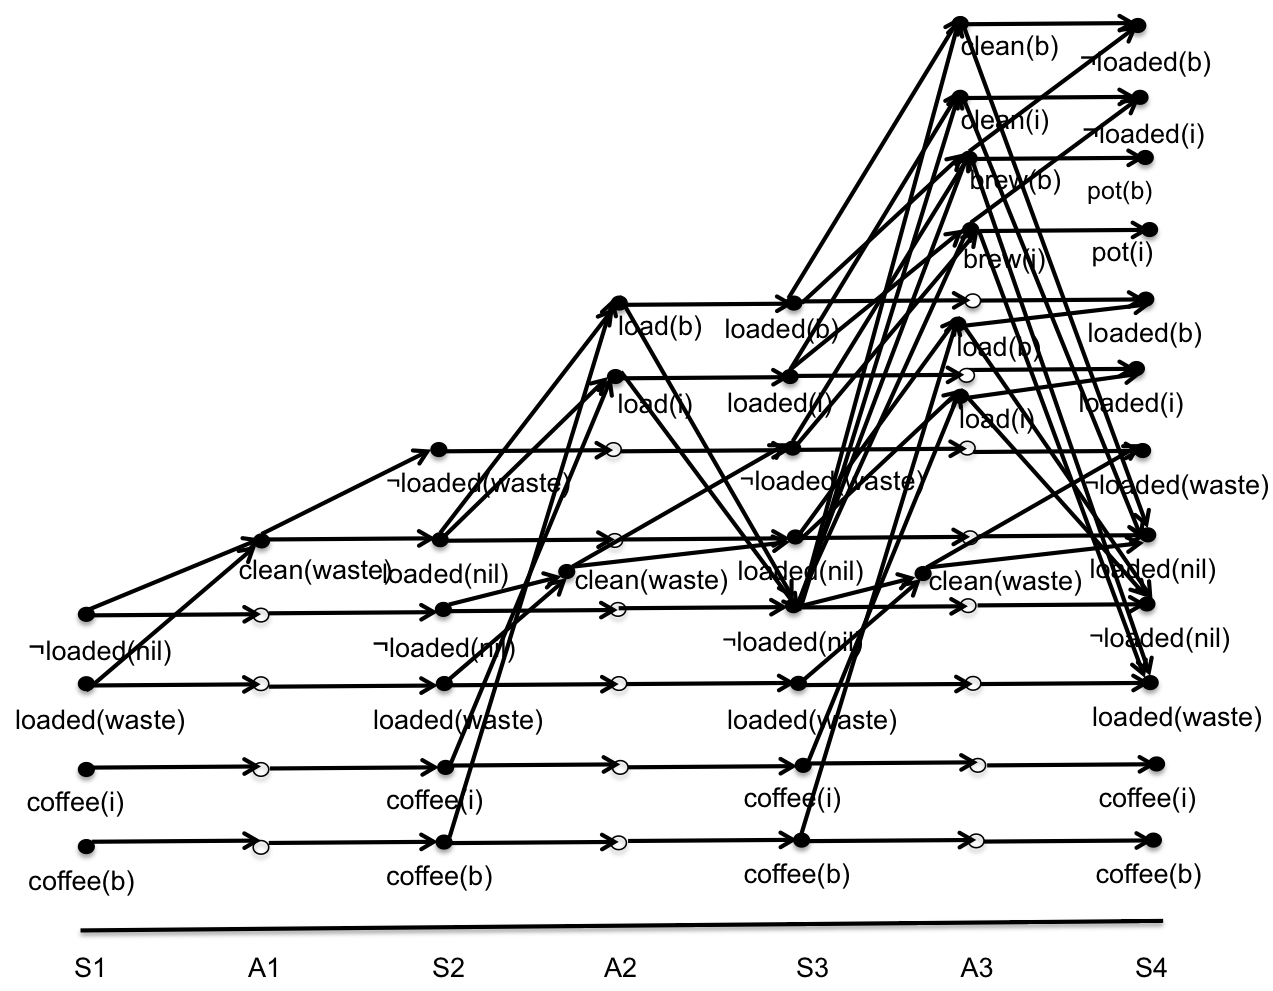
\includegraphics[scale=0.6]{planning.png}
  \caption{Relaxed Planning Graph}
  \label{fig:planninggraph}
\end{center}
\end{figure}
  
  \item (10 pts.) Now make the graph into a standard planning graph by including the mutexes. Indicate the appropriate mutexes at each level. Indicate which type of mutex each is.\\
  
  Since it is hard to see all the types of conflicts in the graph, I list all the conflicts in Figure \ref{fig:planninggraph} as below:
  \begin{itemize}
  	\item  level S2:
  			\begin{itemize}
 				 \item \textbf{Negated Literals:} [ $\neg$loaded(waste), loaded(waste)], [ $\neg$loaded(nil), loaded(nil)]
 				 \item \textbf{Inconsistent Support:}  [ loaded(waste), loaded(nil)], [ $\neg$loaded(waste), $\neg$loaded(nil)]
			\end{itemize}
	\item  level A2: 
			\begin{itemize}
 				 \item \textbf{Inconsistent Effect:} [ clean(waste), load(b) ], [ clean(waste), load(i)], 
 				 \item \textbf{Interference:}  [ load(b), load(i)]
 				 \item \textbf{Competing Needs:} 
			\end{itemize}
	\item  level S3:
  			\begin{itemize}
 				 \item \textbf{Negated Literals:} [ $\neg$loaded(waste), loaded(waste)], [ $\neg$loaded(nil), loaded(nil)]
 				 \item \textbf{Inconsistent Support:}  [ loaded(waste), loaded(nil)], [ loaded(waste), loaded(b)], [ loaded(waste), loaded(i)], 
 				 [ loaded(b), loaded(i)], 
			\end{itemize}
	\item  level A3: 
			\begin{itemize}
 				 \item \textbf{Inconsistent Effect:} [ clean(waste), load(b) ], [ clean(waste), load(i)], 
 				 [clean(b), load(b)],[clean(i), load(i)],[brew(b),load(b)],
 				 [brew(i),load(i)],[brew(b),clean(waste)],[brew(i),clean(waste)]
 				 \item \textbf{Interference:}  [ load(b), load(i) ], [brew(b),brew(i)],[brew(b),clean(b)],[brew(i),clean(i)]
 				 \item \textbf{Competing Needs:}  [brew(b), brew(i)], [clean(b),load(b)], [clean(b),load(i)],
 				 [clean(i),load(b)], [clean(i),load(i)],[brew(b),clean(i)],[brew(i),clean(b)],
 				 
			\end{itemize}
	\item  level S4:
  			\begin{itemize}
 				 \item \textbf{Negated Literals:} [ $\neg$loaded(waste), loaded(waste)], [ $\neg$loaded(nil), loaded(nil)],
 				 [ $\neg$loaded(b), loaded(b)],[ $\neg$loaded(i), loaded(i)]
 				 \item \textbf{Inconsistent Support:}  [ loaded(waste), loaded(nil)], [ loaded(waste), loaded(b)], [ loaded(waste), loaded(i)], 
 				 [ loaded(b), loaded(i)], [pot(b), pot(i)], [pot(b), loaded(b)],[pot(i), loaded(i)],[pot(b),$\neg$loaded(waste) ],
 				 [pot(i),$\neg$loaded(waste) ],[pot(b),loaded(nil) ],[pot(i),loaded(nil) ],[pot(b),loaded(i) ],[pot(i),loaded(b) ]
			\end{itemize}

  \end{itemize}
  
  \item (5 pts.) Avoiding the mutexes, extract a plan from the planning graph in (b).
  
  The plan is [ clean(waste), load(i), brew(i) ]
  
\end{enumerate} 	

 	\item (30 pts.) Consider the following description: There are four animals in the world, by the names of Mufasa, Velocitus Incalculii, Willie, and Woody. Mufasa is a lion, Velocitus Incalculii is a roadrunner, Willie is a whale, and Woody is a woodpecker. Roadrunners and woodpeckers are kinds of birds, while lions and whales are kinds of mammals. All mammals are covered with hair while birds are covered with feathers. As a general rule, mammals can run and birds can fly, but there are exceptions. Whales can swim and not run, and roadrunners can run and not fly, and therefore both are exceptions to the general rules. Lions and woodpeckers are not exceptions. 

Answer the following questions:
	\begin{enumerate}
		\item (5 pts.) Represent the above world description using a semantic network. \\
		
		Figure \ref{fig:sn} shows the semantic network.
		
		\begin{figure}[!iht]
\begin{center}
  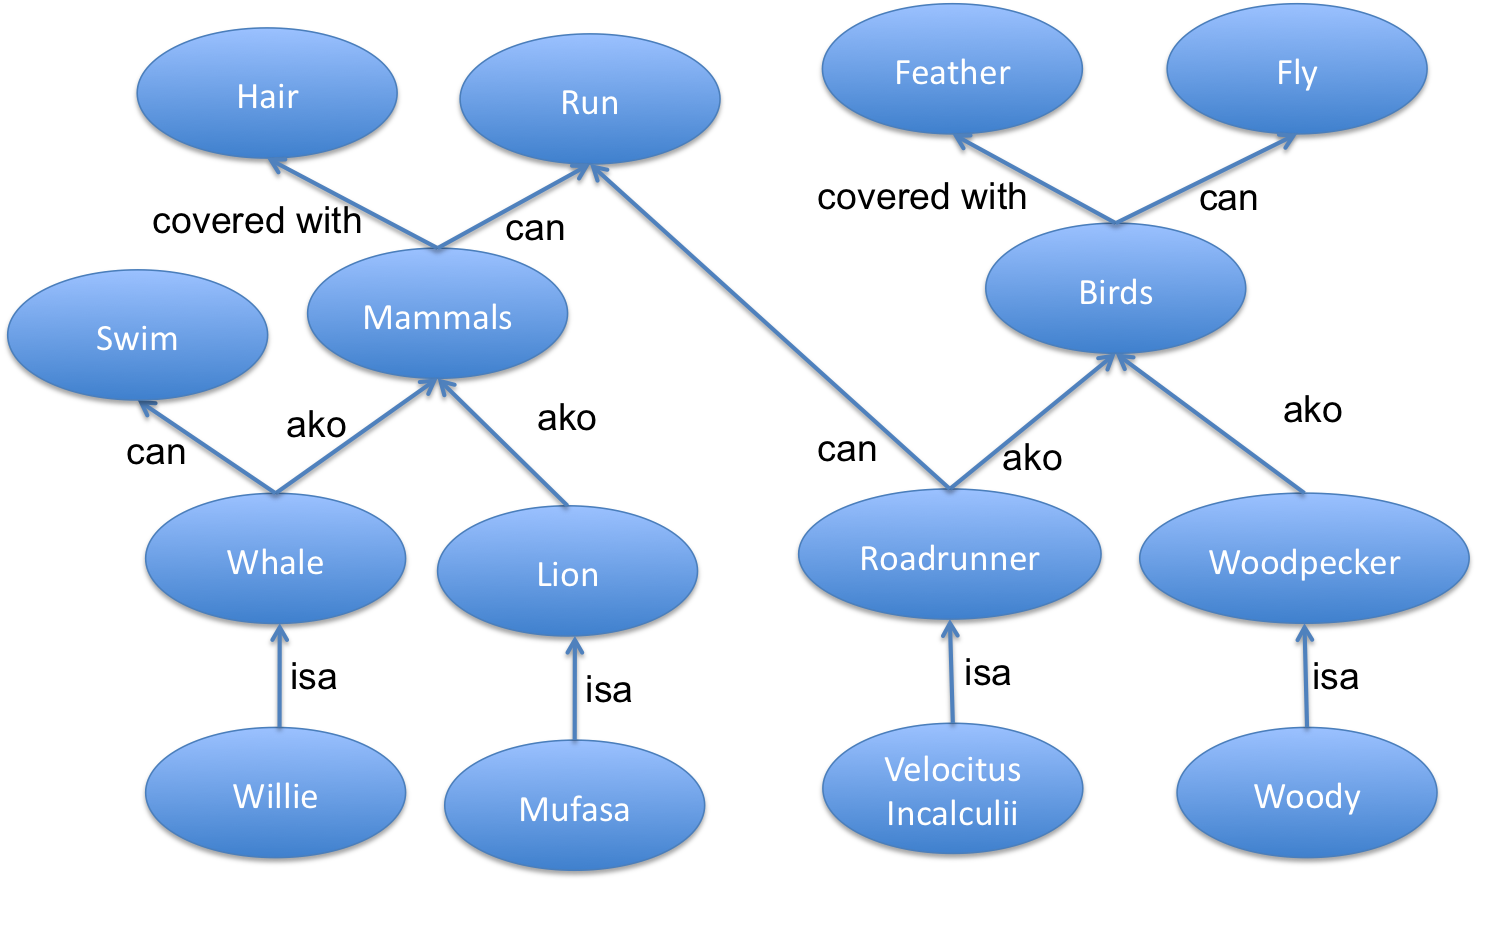
\includegraphics[scale=0.5]{semanticNetwork.png}
  \caption{Semantic Network}
  \label{fig:sn}
\end{center}
\end{figure}
		\item (5 pts.) Implement the semantic net in Prolog. Use a technique patterned on examples in class and webnotes.
		\item (5 pts.) Mufasa is a lion, which is a kind of mammal. Therefore, lion is a mammal. Add a rule to your prolog database that generalizes this to all animals. Run a sample query to demonstrate this rule and show the output.\\
		
		Query: value(lion,isa,X).\\
		Result: X = mammals ; \\
		
		Query: value(roadrunner, isa, X).\\
		Result: X = birds ;\\
		
		\item (10 pts.) Now add rules to the prolog database so that all animal instances inherit the properties of their kind, namely being covered with hair or feathers, running, swimming, or flying. Run a sample query to demonstrate the rules and show the output.\\
		
		Query: value(willie, coveredWith, X).\\
		Result: X = hair ;\\
		
		Query: value(velocitusIncalculii, can, X). \\
		Result: X = run ; X = fly. \\
		
		Query: value(mufasa, can, X).\\
		Result: X = run ;\\
		
		Query: value(woody, coveredWith, X).\\
		Result: X = feather ;\\
		
		
		
		\item (5 pts.) Because your implementation did not account for exceptions, it should conclude that Willie can run and Velocitus Incalculii can fly!! Fix this problem. (Note: While it may be true that road runners can indeed fly, they cannot be airborne for more than a few seconds, and hence for this question consider them non-flying birds.) Show the output to show that you have fixed this problem. \\
		
		Query: value(willie, can, X). \\
		Result: X = swim ; false. \\
		
		Query: value(willie, can, run). \\
		Result: false. \\
		 
		Query: value(whale, can, run). \\
		Result: false. \\
		
		Query: value(velocitusIncalculii, can, X). \\
		Result: X = run ; false. \\
		
		Query: value(velocitusIncalculii, can, fly). \\
		Result: false. \\
		
		Query: value(roadrunner, can, fly). \\
		Result: false. \\
		
		
\end{enumerate}

\textbf{To earn full credit, submit the prolog file, and sample queries and outputs for (c), (d) and (e).}

\item (15 pts.) In a document classification problem, we wish to classify each document in the collection into a predefined set of categories based on the text (or, the words) contained in them. A fairly straightforward way is to use a Naive Bayes classifier where the document is the hypothesis variable and the evidence is the presence (or absence) of the words. We assume that the words occur independently.
	\begin{enumerate}
  		\item (5 pts.) If you were asked to build such a Naive Bayes model, how would you do it, given a training set? (You don't have to actually build anything.)\\
  		
  		Suppose the words are $w_1, w_2, \ldots, w_n$ and the categories of documents are $C_1, C_2, \ldots, C_n$.\\
  		Using a naive bayes classifier to classify documents, we can compute the probability for the categories using the following equations:
  		\begin{equation} P(w_1, w_2, \ldots, w_n, C_i) \end{equation}
  		Since the words occur independently, the above equation is equivalent to:
  		\begin{equation} P(C_i) ( \prod_{k=1}^{n}P(w_k|C_i)) \end{equation}
  		
  		
  		\item (5 pts.) If a new document is presented, explain how it would be classified.
  		If a new document is presented, we first compute the occurences of words in the new document. Assume that the values are $w_1, w_2, \ldots, w_n$. Then, we can compute the probabilities for all the categories using the equation (2) and choose the categories that has the highest probability.
  		
		\item (5 pts.) Is the conditional independence assumption valid for this problem? Explain. 
		
		The condition indenpence assumption may not be valid for this problem. Since for the documents that describes various topics, some words coexists for each topic. For example, for a document describing cardiac diseases, the word ``heart'' and ``cardiac'' may apprear together many times. 
	\end{enumerate}

\item (10 pts.) As a part of a regular health checkup mandated by your insurance company, you undergo a medical check for presence of a particular new virus in your blood. The test is 98\% accurate. Recent statistics show that only a small proportion of the population has the virus (about 1 in 10000). Should you be happy that this is a rare virus? Given a positive test result, what are the chances that you actually have the virus? 

	The population of the earth is about 6.7 billion. Therefore, given the statistics result, there would still be $6,700,000,000 * (\frac{1}{10000})$ =  67,000 people suffering from the virus. Given a positive test result, the chances that you can have the virus can be computed using the following equation if we assume the test result is independent with the probability that people has the virus: 
	\[
	P(actual | test) = P(actual,test)/P(test) = P(actual) = \frac{1}{10000}
	\]


\item (25 pts) Babies have few and simple needs, but they have even fewer ways to communicate those needs to their parents. Parents need some way to figure out what is the matter with their child. Assume we know the following:

P(sick) = .3 \\
P(ache $|$ sick) = .75\\
P(ache $|$ $\neg$sick) = .1\\
P(tired) = .6\\
P(cry $|$ ache, tired) = .9\\
P(cry $|$ ache, $\neg$tired) = .65\\
P(cry $|$ $\neg$ache, tired) = .55\\
P(cry $|$ $\neg$ache, $\neg$tired) = .2\\

	\begin{enumerate}
		\item (5 pts) Assuming that the above conditional probabilities are sufficient to specify the values for a Bayes net for this problem, draw a picture of such a Bayesian network.\\
		
		Figure \ref{fig:bn} shows the bayes network for the babies problem.\\
	
\begin{figure}[!iht]
\begin{center}
  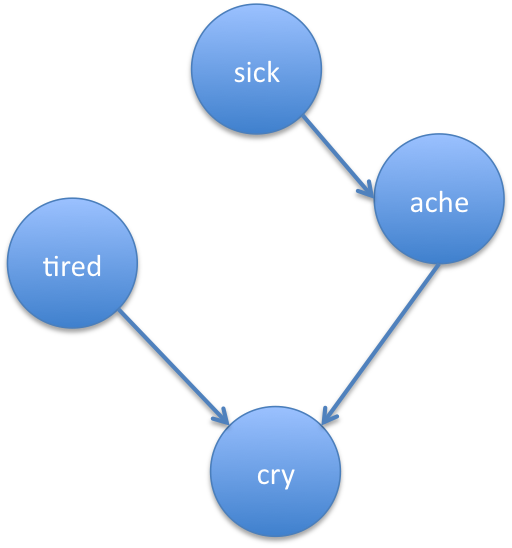
\includegraphics[scale=0.5]{bayesNetwork.png}
  \caption{Bayes Network}
  \label{fig:bn}
  \vspace*{-4ex}
\end{center}
\end{figure}

		\item (20 pts) Compute the full joint probability table for this Bayesian network. Please model your table on the following template:
	\end{enumerate}
	
	\begin{table}[h]
	\centering
	\begin{tabular}{|c|c|c|c|c|c|}
	\hline
	\multicolumn{2}{|c|}{}&\multicolumn{2}{c|}{sick}&\multicolumn{2}{c|}{$\neg$sick} \\ \cline{3-6}
	\multicolumn{2}{|c|}{}&tired&$\neg$tired&tired&$\neg$tired \\ \hline
	ache&cry& 0.1215& 0.0585& 0.0378 & 0.0182\\ \cline{2-6}
	&$\neg$cry& 0.0135&0.0315 &0.0042 & 0.0098\\ \hline
	$\neg$ache&cry& 0.02475 &0.006 & 0.2079& 0.0504\\ \cline{2-6}
	&$\neg$cry& 0.02025&0.024 &0.1701 & 0.2016\\ \hline
	\end{tabular}
	\end{table}
	
	Below are the euqations for the four cells at the first row.
	
	\[
	 \begin{array}{lcl} P(sick, tired, ache, cry)& = &P(sick) * P(tired | sick) * P(ache | sick, tired) * P(cry| sick,tired,ache) \\
 	 						   &=&P(sick) * P(tired) * P(ache|sick) * P(cry|ache,tired) \\
 	 						   &=&0.3*0.6 *0.75*0.90\\
 	 						   &=&0.1215 
 	 \end{array}	 
 	 \]
 	 
 	 \[
	 \begin{array}{lcl} P(sick, \neg tired, ache, cry)& = &P(sick) * P(\neg tired | sick) * P(ache | sick, \neg tired) * P(cry| sick,\neg tired,ache) \\
 	 						   &=&P(sick) * P(\neg tired) * P(ache|sick) * P(cry|ache,\neg tired) \\
 	 						   &=&0.3*0.4 *0.75*0.65\\
 	 						   &=&0.0585
 	 \end{array}	 
 	 \]
 	 
 	 
	\[
	 \begin{array}{lcl} P(\neg sick, tired, ache, cry)& = &P(\neg sick) * P(tired | \neg sick) * P(ache | \neg sick, tired) * P(cry| \neg sick,tired,ache) \\
 	 						   &=&P(\neg sick) * P(tired) * P(ache|\neg sick) * P(cry|ache,tired) \\
 	 						   &=&0.7*0.6 *0.1*0.9\\
 	 						   &=&0.0378 
 	 \end{array}	 
 	 \]
 	 
 	 \[
	 \begin{array}{lcl} P(\neg sick, \neg tired, ache, cry)& = &P(\neg sick) * P(\neg tired | \neg sick) * P(ache | \neg sick, \neg tired) * P(cry| \neg sick,\neg tired,ache) \\
 	 						   &=&P(\neg sick) * P(\neg tired) * P(ache|\neg sick) * P(cry|ache,\neg tired) \\
 	 						   &=&0.7*0.4 *0.1*0.65\\
 	 						   &=&0.0182
 	 \end{array}	 
 	 \]
 	 
% 							   =0.3*0.4*0.75*0.65
%							   =0.7
\end{enumerate}
\end{document}
